%! Author = mariuszindel
%! Date = 02.11.20

\section{.Net Grundlagen}
\subsection{Überblick}
    Es wird grundsätzlich zwischen \textcolor{OSTPink}{.NET Framework} und \textcolor{OSTPink}{.NET Core} unterschieden.
\subsubsection{Geschichtliches}
    \vspace{-10pt}
    \begin{multicols}{2}
    \textbf{\textcolor{OSTPink}{.NET Framework}}
    \begin{itemize}
        \item Ursprüngliches Framework
        \item Seit 2002
        \item Läuft nur unter Windows
        \item Open Source seit 2008
        \item End of Life seit Version 4.8
    \end{itemize}

    \columnbreak

    \textbf{\textcolor{OSTPink}{.NET Core}}

    \begin{itemize}
        \item Neuimplementation seit 2016
        \item Plattform-neutral
        \item OpenSource
        \item Zukünftiger Weg
    \end{itemize}
    \end{multicols}

\subsubsection{Bestandteile}
    \vspace{-10pt}
\begin{multicols}{2}
    \textbf{\textcolor{OSTPink}{CommonLanguageRuntime}}
    \begin{itemize}
        \item Mächtige Laufzeitumgebung ähnlich (JVM)
        \item Common Type System (CTS) $\rightarrow$ Typensystem für alle .NET-Sprachen
        \item Common Language Specification (CLS) $\rightarrow$ Sprach-Eigenschaften für alle .NET-Sprachen
    \end{itemize}

    \columnbreak

    \textbf{\textcolor{OSTPink}{.NETClassLibrary}}

    \begin{itemize}
        \item Basis Klassen
        \item Klassen für DB-Zugriff
        \item Klassen für XML, Dateisystem
        \item Klassen für Windows-GUIs
    \end{itemize}
    \end{multicols}
\vspace{-8pt}
\subsubsection{.NET Architektur}
\begin{center}
    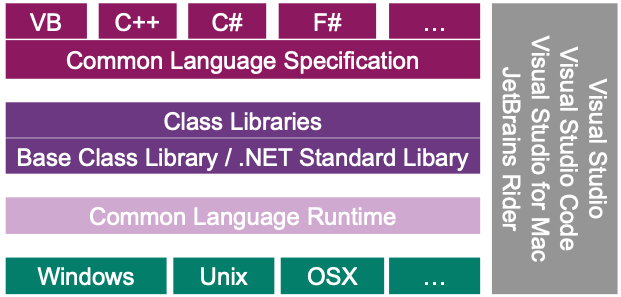
\includegraphics[scale=0.28]{graphic/grundlagen/Grundlagen_dotNET Architektur.png}
\end{center}
\vspace{-8pt}


\subsection{Common Language Runtime(CLR)}
Die CLR ist eine Laufzeitumgebung für .NET-Code, welche ähnlich wie die JVM bei Java ist. Sie umfasst Funktionen wie:\\
\begin{multicols}{2}
\begin{itemize}
    \item JIT-Compilers für die Übersetzung von Intermediate Language Code in Maschinencode
    \item Class Loader für das Laden von Klassen-Code zur Laufzeit
    \item Garbage Collection
    \item Code Access Security
    \item Sprachübergreifendes Debugging
    \item Exceptions
    \item Type Checking und Code Verifikation des IL-Codes
    \item Thread-Verwaltung
    \item Basis-Klassen mit System-Funktionen
\end{itemize}
\end{multicols}

\subsubsection{CLR Architektur}
Die Programmiersprache Visual Basic, C\# sowie C++ werden von einenm Compiler in einen IL Code übersetzt.
Anschliessend wird der IL Code durch die JIT Compiler der Common Language Runtime in eine exe oder dll übersetzt (Maschinencode)
\vspace{-8pt}
\begin{center}
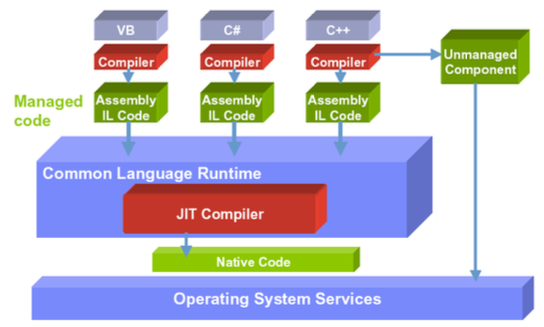
\includegraphics[scale=0.3]{graphic/grundlagen/Grundlagen_CLR Architetktur}
\end{center}

\subsection{Microsoft Intermediate Language (MSIL)}
Die Microsoft Intermediate Language ist eine vorkompilierte Zwischensprache und Prozessor-unabhängig.
Die Sprache an sich selbst sieht sehr Assemblermässig aus.\\
\begin{enumerate}
   \item Portabilität $\rightarrow$ z.B. Nicht-Intel-Prozessoren / Unix / etc.
   \item Typsicherheit $\rightarrow$ Beim Laden des Code können Typen- Sicherheits- und weitere Security-Checks durchgeführt werden.
\end{enumerate}

\begin{enumerate}
   \item Laufzeiteffizienz $\rightarrow$ (kann wettgemacht werden durch JIT-Compiler, welcher zur Laufzeit den Prozessortyp erkennt und spezifische Maschineninstruktionen ausnutzen kann)
\end{enumerate}

    \begin{center}
    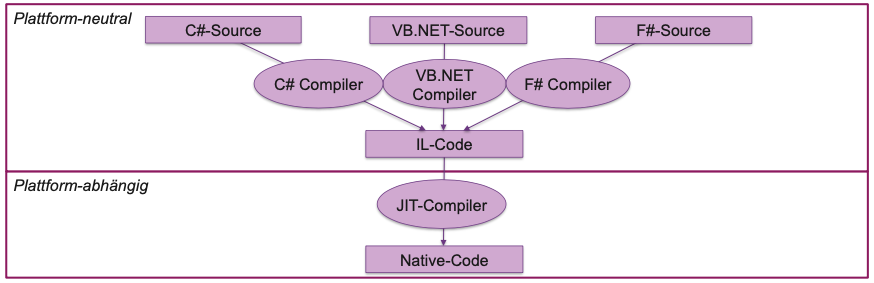
\includegraphics[scale=0.28]{graphic/grundlagen/Grundlagen_MSIL.png}
    \end{center}


\subsubsection{Just in Time (JIT) Compiler}

Die bereits übersetzten Methoden sind in der Grafik mit (ASM) bezeichnet.
Die restlichen Methoden stehen noch als IL Code zur verfügung.
Es wird die Methode 1 in Klasse A ausgeführt.
Diese ruft die Methode 1 in der Klasse B auf.
Anschliessend wird erkannt, dass die Methode 1 in B noch nicht übersetzt wurde.
Der JIT Compiler übersetzt diese Methode dann und übersetzt den IL Code und ersetzt diesen durch Assembler Code.
\begin{center}
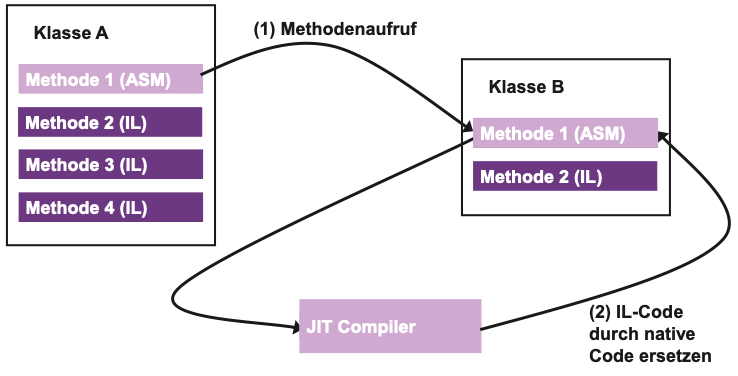
\includegraphics[scale=0.28]{graphic/grundlagen/Grundlagen_JIT Compile.png}
\end{center}


\subsection{Assemblies}
\begin{multicols}{2}
\begin{itemize}
    \item Kompilation erzeugt Assemblies
    \item Deployment- und Ausführungs-Einheit
    \item Executable (*.exe) oder Library (*.dll)
    \item Dynamisch ladbar
    \item Definiert Typ-Scope
    \item Kleinste versionierbare Einheit
\end{itemize}
\end{multicols}

\subsubsection{Überblick}
Ein Assembly besteht hauptsächlich aus 3 Komponenten:





\begin{tabular}{p{2.4cm} | p{2.4cm} | p{2.4cm}}
    \textcolor{OSTPink}{Manifest} & \textcolor{OSTPink}{Module} & \textcolor{OSTPink}{Resourcen}\\
    \hline
    Referenzen $\rightarrow$ welche weiteren Assemblys dieses referenzieren&0 bis n Stück (Können Klassen, Interfaces, Enumerationen, etc. sein)&Bilder, etc.\\
    Metadaten für Klassen und Ressourcen&Typ aus MSIL Code&\\
    Infos $\rightarrow$ Versionsdaten und Autoren Infos& Metadaten (public, abstract etc)&\\
\end{tabular}
\vspace{-8pt}
\begin{center}
\includegraphics[scale=0.3]{graphic/grundlagen/Grundlagen_Assemblies Überblick.png}
\end{center}
\vspace{-8pt}

\subsection{CommonTypeSystem}
\subsubsection{Überblick}
CLR hat ein integriertes Typen-System
\begin{itemize}
    \item Einheitliches Typensystem für alle .NET-Programmiersprachen
    \item Typen in Laufzeitsystem definiert, nicht in Programmiersprache
    \item Alle Typen sind von System.Object abgeleitet
    \item Reference- und Value-Types (int, long, bool, etc.)
    \item Automatische Umwandlung (Value Types – Reference Types)
\end{itemize}

\subsection{Reference- \& Value Types}
    \begin{tabular}{| p{2.5cm}  p{2.5cm} | p{2.5cm}|}

        \hline
        &Reference (Class)&Value(Struct)\\
        \hline
        \hline
        Speicherort&Heap&Stack\\
        \hline
        Variable enthält&Objekt-Referenz&Wert\\
        \hline
        Nullwerte&Möglich&Nie\\
        \hline
        Default value&null&0|false|'\textbackslash0'\\
        \hline
        Methodenaufruf&Kopiert Referenz& Kopiert Wert\\
        \hline
        Ableitung möglich&Ja&Nein (sealed)\\
        \hline
    \end{tabular}




\subsubsection{Reference Types}

    \begin{itemize}
        \item Auf dem Heap gespeichert
        \item Variable enthält Referenz
        \item Garbage Collected
        \item Konstruktor erzeugt \& initialisiert Objekt
        \item Objekt hat Referenz auf seine Typenbeschreibung
    \end{itemize}
\vspace{-8pt}
\begin{center}
    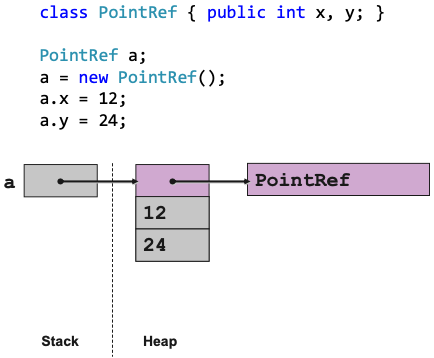
\includegraphics[scale=0.35]{graphic/grundlagen/Grundlagen_Reference Types.png}
\end{center}
\vspace{-8pt}

\subsubsection{Value Types}

\begin{itemize}
    \item Zur Speicherung Roher Werte
    \item Auf Stack abgelegt
    \item Konstruktur macht nur Initialisierung
    \item sealed
    \item Boxing $\rightarrow$ Automatische Umwandlung in Reference Type
    \item Unboxing $\rightarrow$ Automatische Rückumwandlung in Value Type
    \item Effizienter Zugriff
    \item Keine Garbage Collection nötig
    \end{itemize}

\begin{center}
    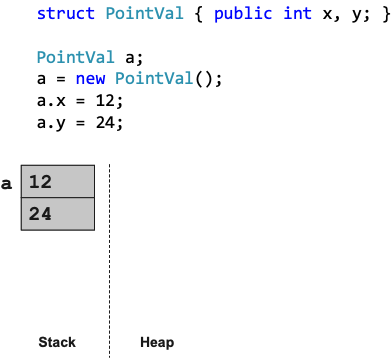
\includegraphics[scale=0.35]{graphic/grundlagen/Grundlagen_Value Types.png}
\end{center}



\subsection{Boxing \& Unboxing}
Vorab den Wert speichern als int:
\begin{lstlisting}
System.Int32 i1 = 123;
\end{lstlisting}


\subsubsection{Boxing}
Kopiert Value Type in einen Reference Type.
\begin{lstlisting}
System.Object obj = i1;
\end{lstlisting}


\subsubsection{Unboxing}
Kopiert Reference Type in einen Value Type.
\begin{lstlisting}
System.Int32 i2 = (System.Int32)obj;
\end{lstlisting}

\vspace{10pt}

Zusammengefasst sieht das ganze Grafisch so aus:
\begin{center}
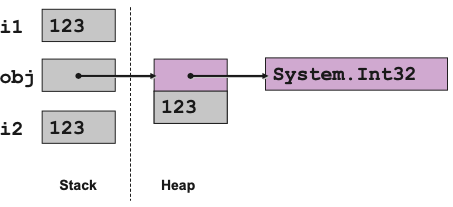
\includegraphics[scale=0.4]{graphic/grundlagen/Grundlagen_Boxing und Unboxing}
\end{center}


\newpage